\documentclass[linenumbers,trackchanges]{aastex7}

\usepackage{graphicx}  % For including images
\usepackage{float}     % For forcing figure placement

% Flowgraphb%
\usepackage{tikz}
\usetikzlibrary{shapes.geometric, arrows}
\tikzstyle{startstop} = [rectangle, rounded corners, minimum width=3cm, minimum height=1cm,text centered, draw=black, fill=white]
\tikzstyle{process} = [rectangle, minimum width=3cm, minimum height=1cm, text centered, draw=black, fill=white]
\tikzstyle{decision} = [diamond, minimum width=3cm, minimum height=1cm, text centered, draw=black, fill=white]
\tikzstyle{arrow} = [thick,->,>=stealth]

\newcommand{\vdag}{(v)^\dagger}
\newcommand\aastex{AAS\TeX}
\newcommand\latex{La\TeX}

\begin{document}

\title{Modeling Dynamical Friction-based Angular Momentum Evolution}


\author{Thomas Joyce}
\altaffiliation{Steward Observatory}
\affiliation{University of Arizona}
\email[show]{thomasajoyce@arizona.edu}  

\section{Introduction} % 1

\sloppy % Justified with no hyphens

\hspace{\parindent} Dynamical friction is a phenomenon resulting from the gravitational scattering of mass particles (for example: stars in a galaxy) from a perturber that acts upon a system to induce angular momentum and energy transfer. This process is prevalent throughout our universe as many galaxies and systems, not just our own, have satellite galaxies, globular clusters, or otherwise massive systems influencing the host's dynamical evolution \citep{Binney_Tremaine-2008}. This direct gravitational influence on galactic structure and orbital dynamics can reveal much about the system's evolution as a whole, and can pave the way for more refined simulation environments predicting the outcomes of galactic interactions and mergers!

\vspace{10pt}

\hspace{\parindent} The study of dynamical friction is crucial to the development of galaxy evolution theories. For example, dynamical friction slows down both the host and satellite galaxies, influencing merge timescales, and as a direct result, the mass growth timescales. Additionally, the satellites affected by dynamical friction will slow and potentially be subject to tidal stripping. This changes the morphology of galaxies and causes regions of over-density and under-density leading to star formation and quenching, as a result. These important dynamical interactions can change the internal kinematics of both the host and satellite galaxies leading to a variety of interesting evolutionary effects to be studied!

\vspace{10pt}

\hspace{\parindent} The understanding of dynamical friction is a complicated one, as it's impossible to observe it playing out in real-time. Astronomers do have the capability of surveying a variety of galaxies at different stages of stability and mergers, however with each system differing by a variable degree, it may be difficult to quantify. Instead, Astronomers must rely on simulations based on real-life mass estimates and observations, where these complex interactions can be modeled and propagated in time to observe the effects. One such experiment even found the existence of dark matter wakes as a result of dynamical friction, fueled by the changing resonance patterns of the satellite's orbit around its host. Garavito-Camargo et al's investigation into DM wakes found that satellites orbiting within the dark matter halos of the host galaxy have the potential to cause these dark matter interactions by presenting density variations in their structure \citep{Garavito-Camargo_2019}. Overall scientists continue to work on developing their understanding of the dynamical friction processes but currently consider the effects of large bodies, such as galaxies and their satellites under the guise of DM-dominated systems. This means that the observations acquired must show a result of these interactions through the analysis of bulge and stellar disk stars, observable as baryonic matter.  

\vspace{10pt}

\hspace{\parindent} However our current understanding of dynamical friction is incomplete as galaxies with bar structures are influenced by these effects as well, and whose evolution can be difficult to model without specific approximations made like that of Rimpei's study \citep{RimpeiChiba}. Additionally, the small-scale interactions proposed by current "fuzzy" DM theories have yet to be fully understood along with their dynamical friction ramifications \citep{Lancaster_2020}. In general, the theory of dynamical friction is fairly well understood in "well-behaved" large scale interactions between massive galaxies and their perturbers, but with edge cases proving more common with increased observations, these questions will be necessary to investigate to gain a fuller understanding. 


\begin{figure}[H]
    \centering
    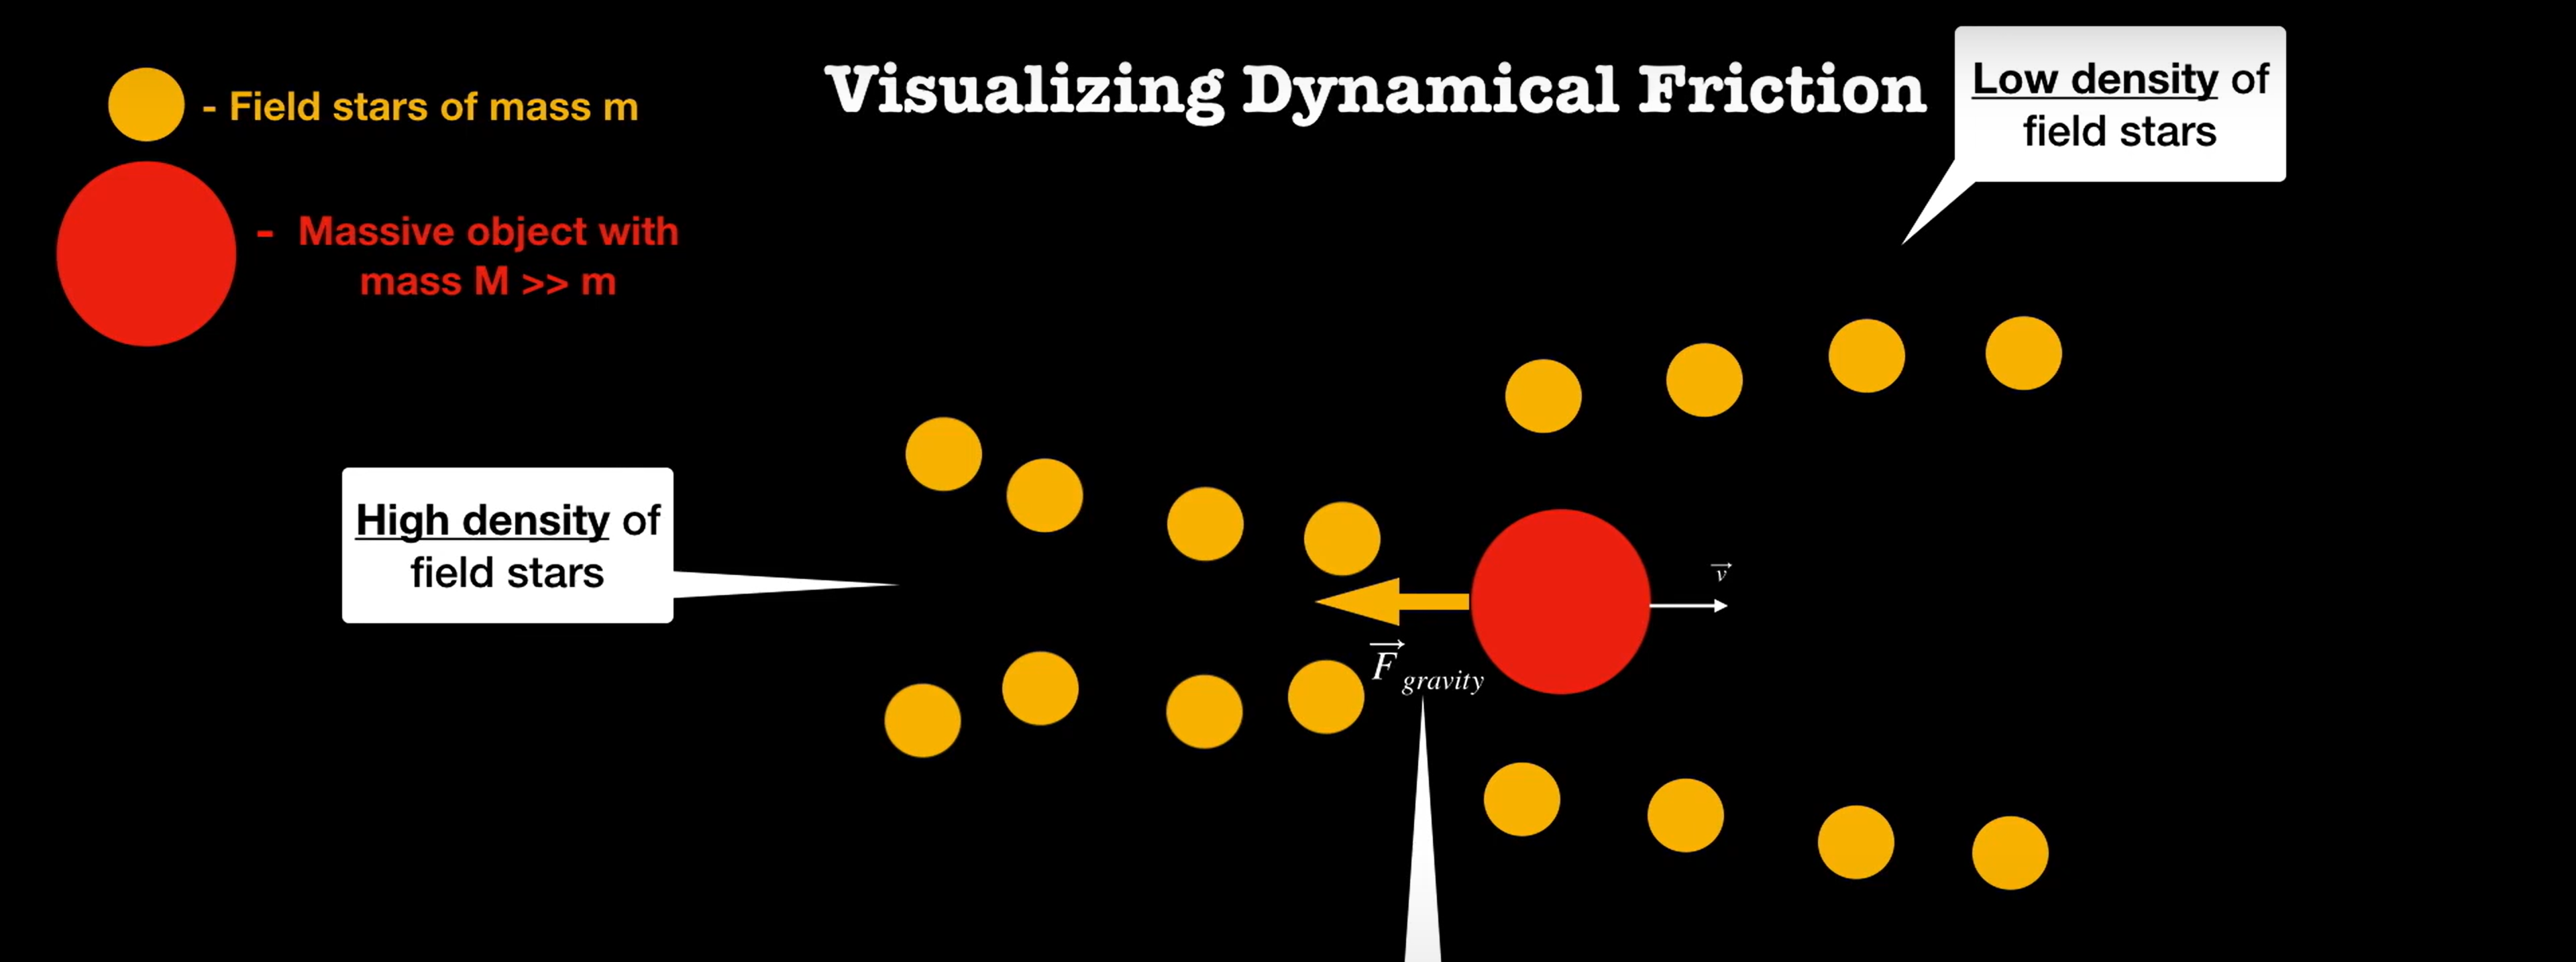
\includegraphics[width=1\linewidth]{Screenshot (71)-cropped.png}
    \caption{Simplified visual example of dynamical friction \citep{Kabasares_2021}.}
    \label{fig:enter-label}
\end{figure}





%%% PAGE BREAK %%%
\newpage
%%% PAGE BREAK %%%

% figure out this nonsense as well
%\title{Dynamical Friction Modeling}
%\author{Thomas Joyce}
%\date{February 22nd, 2025}

%\maketitle

\section{Proposal}

\subsection{This Proposal} % 2.1

For this investigation, I will analyze how angular momentum evolves in time due to the merging of the Milky Way (MW) and M31 systems. I will do so for each particle type (bulge, disk, and DM), and then determine the total angular momentum evolution for each system. Due to dynamical friction the orbits will decay as the angular momentum of the satellite (M31) will substantially decrease. I will utilize the MW, M31, and M33 merging simulation developed by \cite{vandermarel2012} to accomplish this.


\subsection{Methods} % 2.2

To determine the dynamical friction effects on angular momentum, I will need to consider the effects of each galaxy. First I will build an algorithm to find the center of mass reference frame for a particle type. Relative to the center of mass point, I can compute the angular momentum contribution of each particle of a specific type. Then I can iterate this algorithm for each particle type and combine my results to see how each type's angular momentum evolves in time and that of the total system. I can then repeat this for the other galaxy. 

\vspace{10pt}

An Important consideration to take into account is whenever the system begins merging. Here I will need to consider a smaller region, say a specified radius (ex: 10kpc) where I will find the angular momentum of particles within this range. This biasing radius will remove any wild contributions from particles being flung away due to the merger, or any particles that may not be that of the specific galaxy. This way we may only consider the particles most likely to be from the host galaxy being computed. 


\subsection{Hypothesis} % 2.3

I hypothesize that the total system's angular momentum will stay constant throughout this entire simulation. However, the angular momentum of the satellite galaxy (M31) will decrease over time and transfer that momentum to the host galaxy (MW), as a result of dynamical friction.

%%% PAGE BREAK %%%
\newpage
%%% PAGE BREAK %%%

\begin{figure}[H]
    \centering
    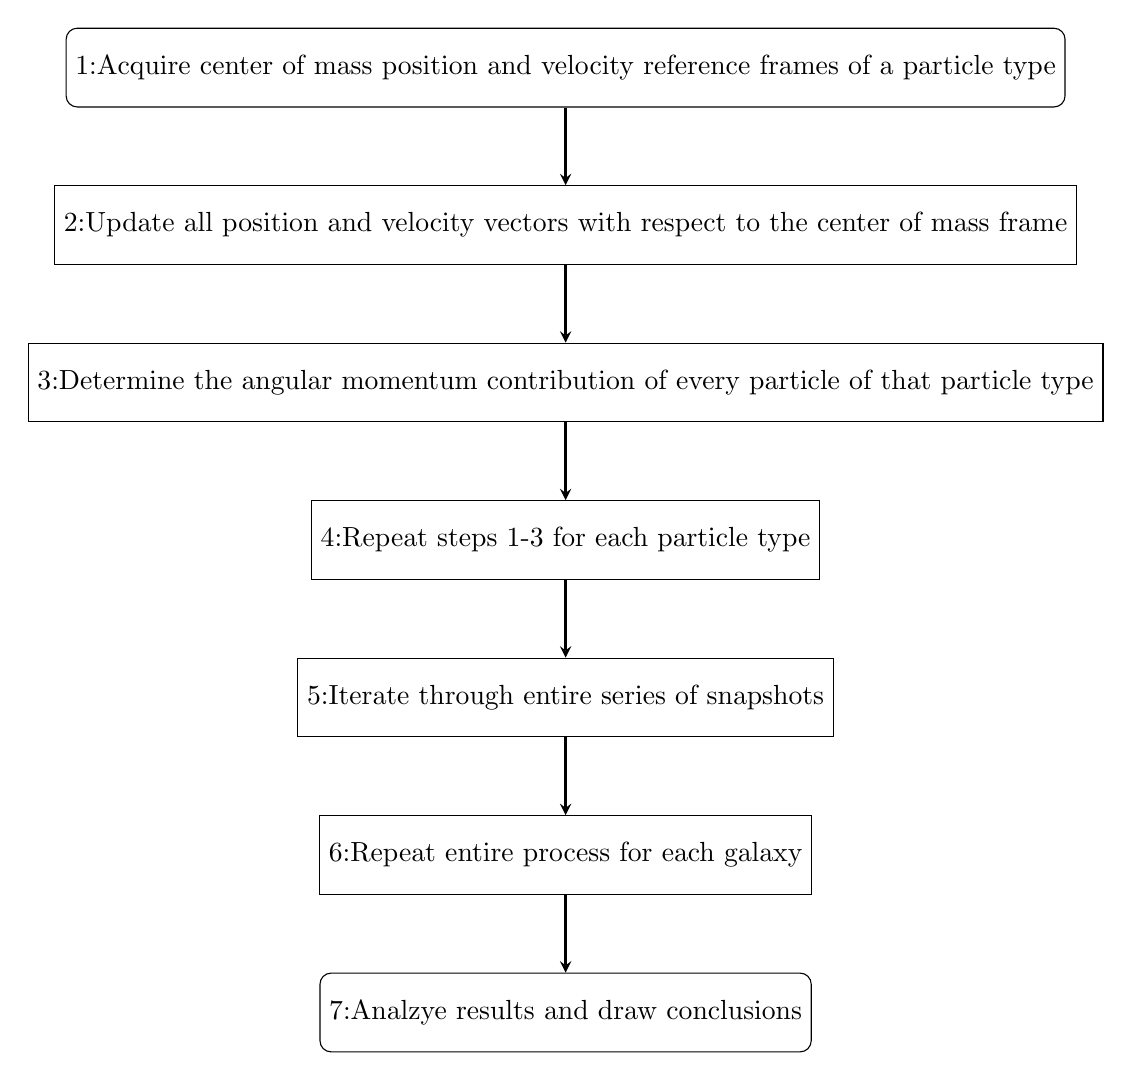
\begin{tikzpicture}[node distance=2cm]
        
        \node (start) [startstop] {1:Acquire center of mass position and velocity reference frames of a particle type};
        \node (step1) [process, below of=start] {2:Update all position and velocity vectors with respect to the center of mass frame};
        \node (step2) [process, below of=step1] {3:Determine the angular momentum contribution of every particle of that particle type};
        \node (step3) [process, below of=step2] {4:Repeat steps 1-3 for each particle type};
        \node (step4) [process, below of=step3] {5:Iterate through entire series of snapshots};
        \node (step5) [process, below of=step4] {6:Repeat entire process for each galaxy};
        \node (end) [startstop, below of=step5] {7:Analzye results and draw conclusions};

        \draw [arrow] (start) -- (step1);
        \draw [arrow] (step1) -- (step2);
        \draw [arrow] (step2) -- (step3);
        \draw [arrow] (step3) -- (step4);
        \draw [arrow] (step4) -- (step5);
        \draw [arrow] (step5) -- (end);
    \end{tikzpicture}
    \caption{Methodology visualized through a flowchart, documenting each step of the experiment.}
    \label{fig:code-flowchart}
\end{figure}





% References %
\bibliographystyle{aasjournal}
\bibliography{Citations}

\end{document}